\documentclass{beamer}
\usepackage{graphicx}
\usepackage{listings}
\usepackage{tikz}
\usetikzlibrary{positioning, arrows.meta, shapes, calc, shapes.multipart}

\title{Introducing Qubes Air design}
\author{Marek Marczykowski-Górecki and Frédéric Pierret}
\date{September 20, 2024}

\begin{document}

\frame{\titlepage}


\begin{frame}{Overview}
    \begin{itemize}
		\item https://www.qubes-os.org/news/2018/01/22/qubes-air/
        \item Understanding communication between Qubes OS hosts.
        \item Different classes involved in the communication process.
        \item RPC requests and policy processing.
        \item Relay mechanisms for remote communication.
		\item https://github.com/QubesOS/qubes-issues/issues/9015
		\item First POC in Qubes Summit 2022!\footnote{https://gist.github.com/fepitre/7af571bbc9de86824e543e2fd49be0aa}
    \end{itemize}
\end{frame}

\begin{frame}{Introducing RemoteVM class}
    \begin{itemize}
        \item \textbf{What is a RemoteVM?}
        \begin{itemize}
            \item A general term for a system that can receive RPC requests from a local Qubes OS environment, but it is hosted remotely.
            \item Can be a qube on a remote Qubes OS host or system, such as:
            \begin{itemize}
                \item Standard Linux or Windows machines,
                \item KVM-based virtual machines,
                \item Devices with different architectures (e.g. Raspberry Pi).
            \end{itemize}
        \end{itemize}
    \end{itemize}
\end{frame}

\begin{frame}{Introducing RelayVM class}
    \begin{itemize}
        \item \textbf{What is a RelayVM?}
        \begin{itemize}
            \item A specialized LocalVM (formerly known as QubesVM) or a RemoteVM that acts as a bridge between the local and remote Qubes OS hosts.
            \item Responsible for forwarding RPC requests between a \textbf{RelayVM} (on the local host) and another \textbf{RelayVM} (on the remote host).
			\item Forwarding RPC requests is made with a given \texttt{TRANSPORT\_RPC} service:
			\begin{itemize}
				\item qubesair.SSHProxy
				\item qubesair.WireguardProxy
				\item ...
			\end{itemize}
        \end{itemize}
    \end{itemize}
\end{frame}

\begin{frame}{General Case}
    \begin{itemize}
        \item Communication sequence between local and remote QubesOS:
    \end{itemize}
    \begin{center}
        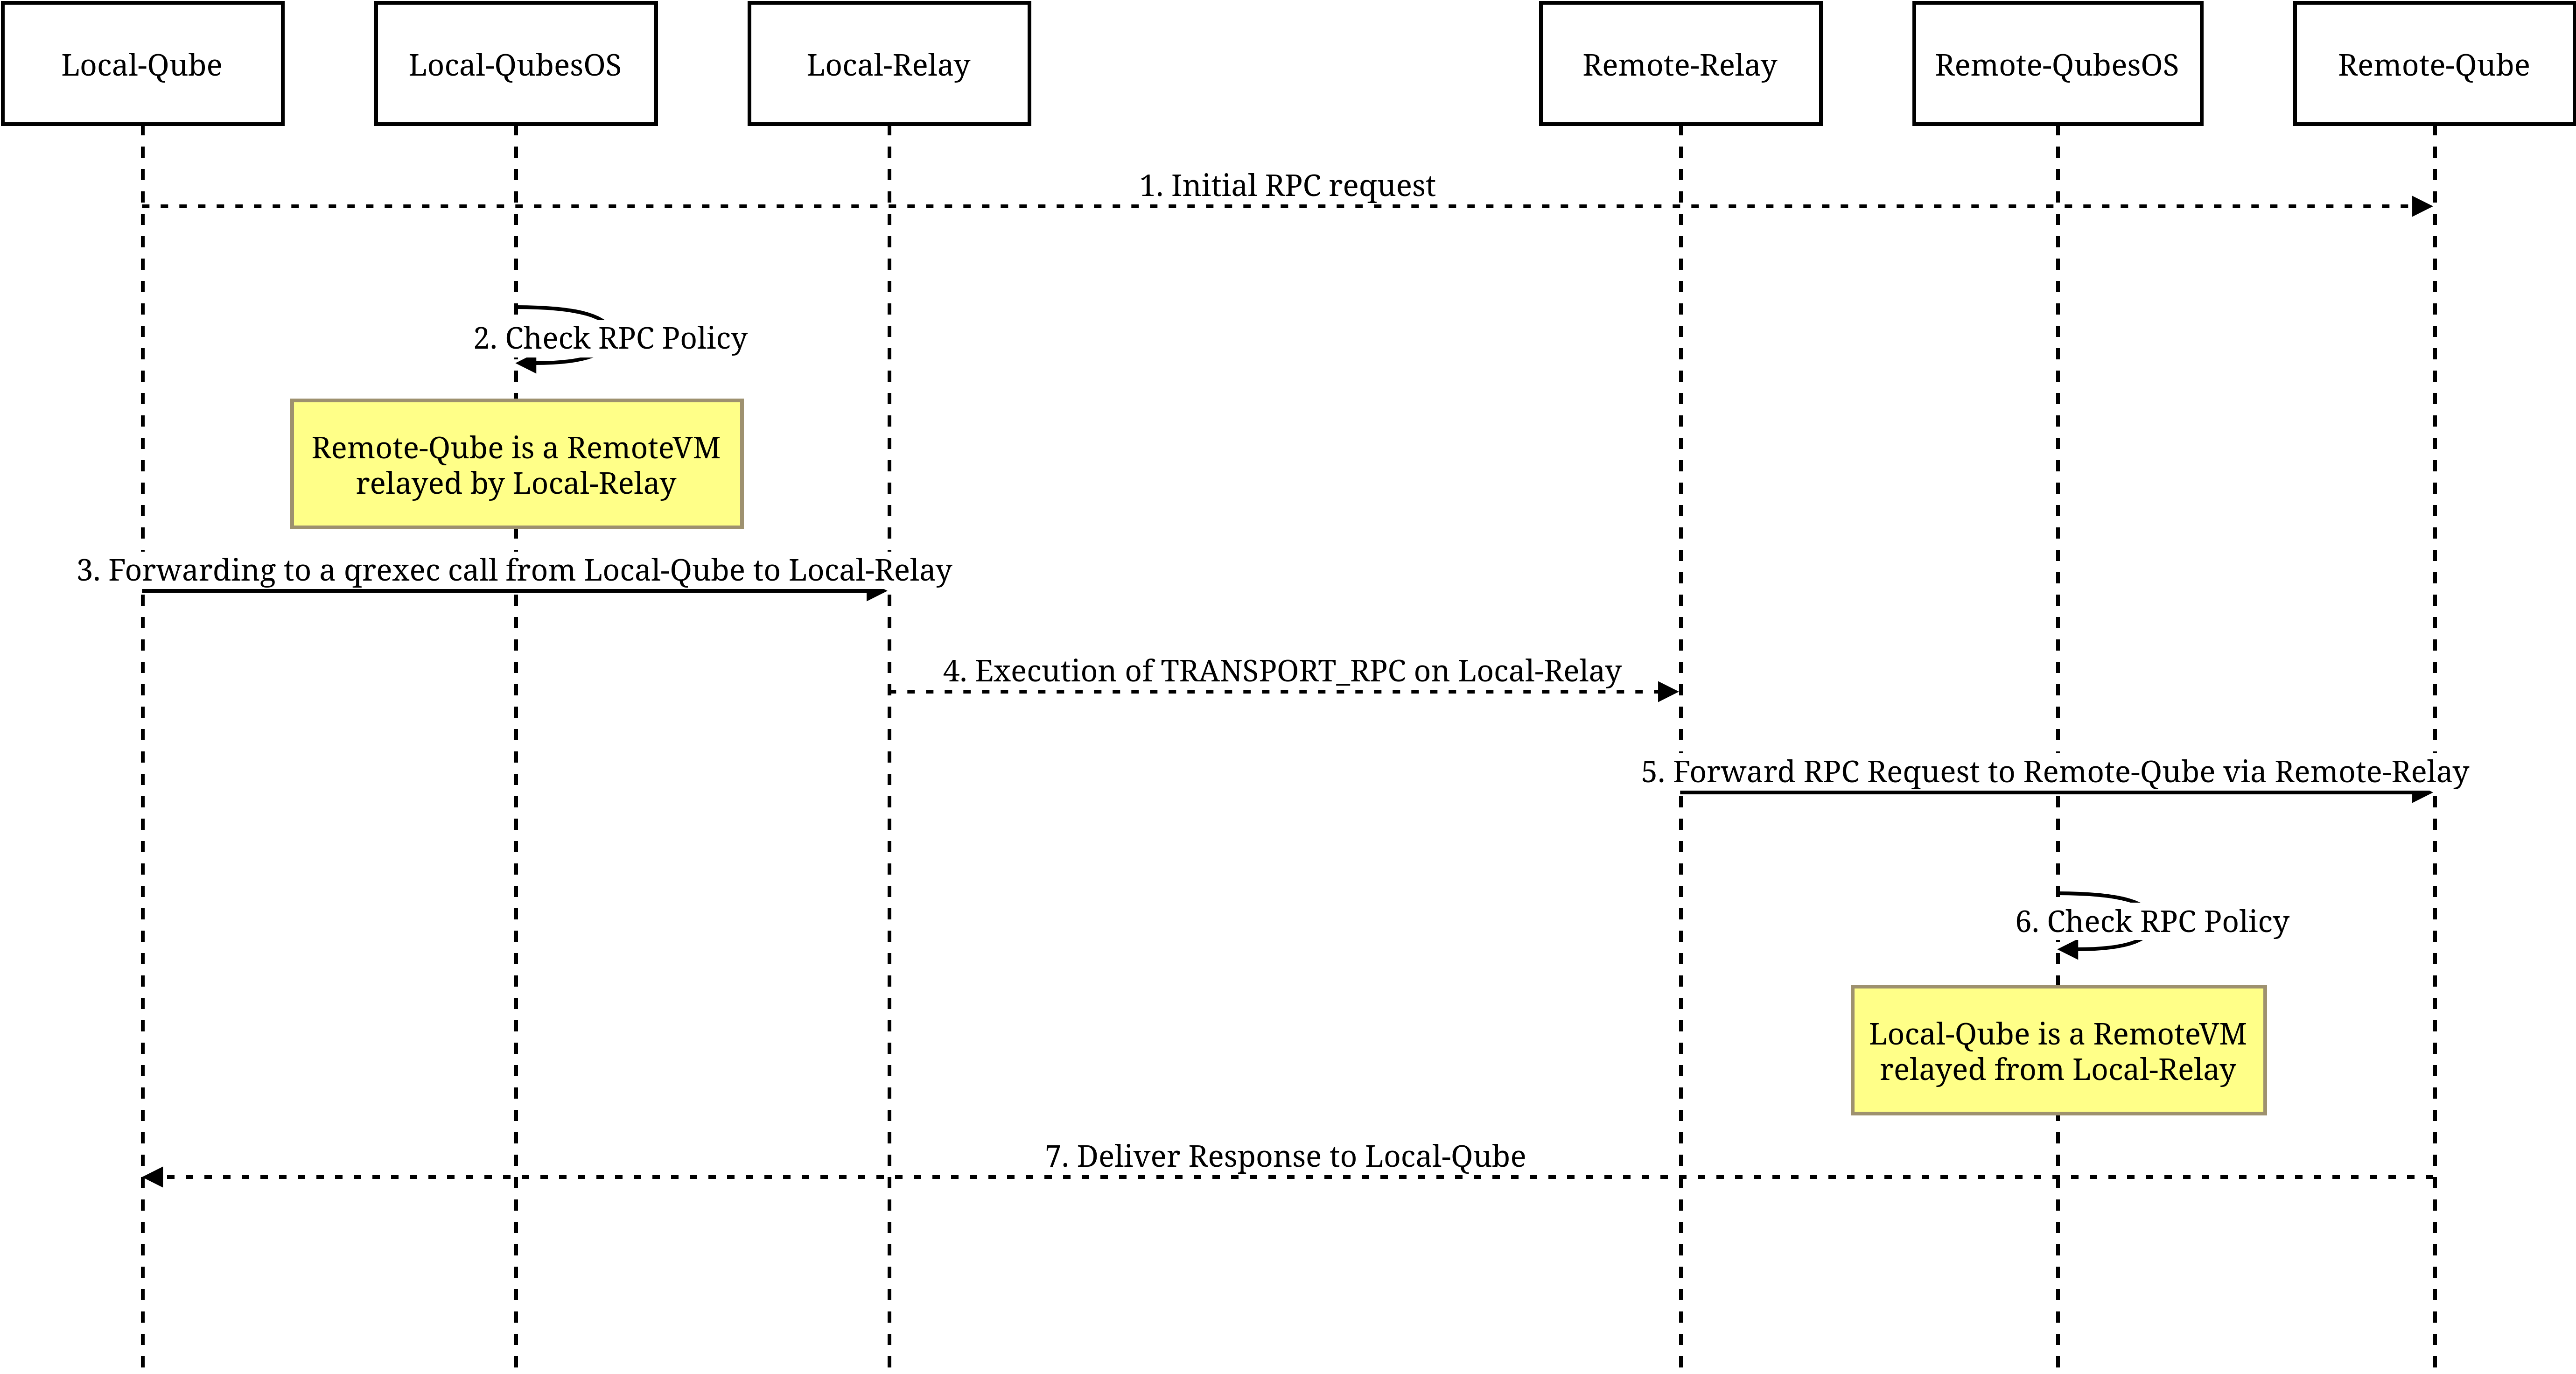
\includegraphics[width=\linewidth]{general.png}
    \end{center}
\end{frame}

\begin{frame}{General Communication Workflow}
    \begin{enumerate}
        \item \textbf{Local-Qube} initiates an RPC request to \textbf{Remote-Qube} (a \textbf{RemoteVM}).
        \item \textbf{Local-QubesOS} checks the RPC policy and routes the request through \textbf{Local-Relay}.
        \item \textbf{Local-Relay} invokes \textbf{TRANSPORT\_RPC} to forward the request to \texttt{Remote-Relay}.
        \item \textbf{Remote-Relay} forwards the request to \textbf{Remote-Qube}.
        \item \textbf{Remote-QubesOS} processes the request, checks policies, and returns the response.
    \end{enumerate}
\end{frame}

\begin{frame}{Particular Case: Non-QubesOS Host RemoteVM}
	\begin{center}
        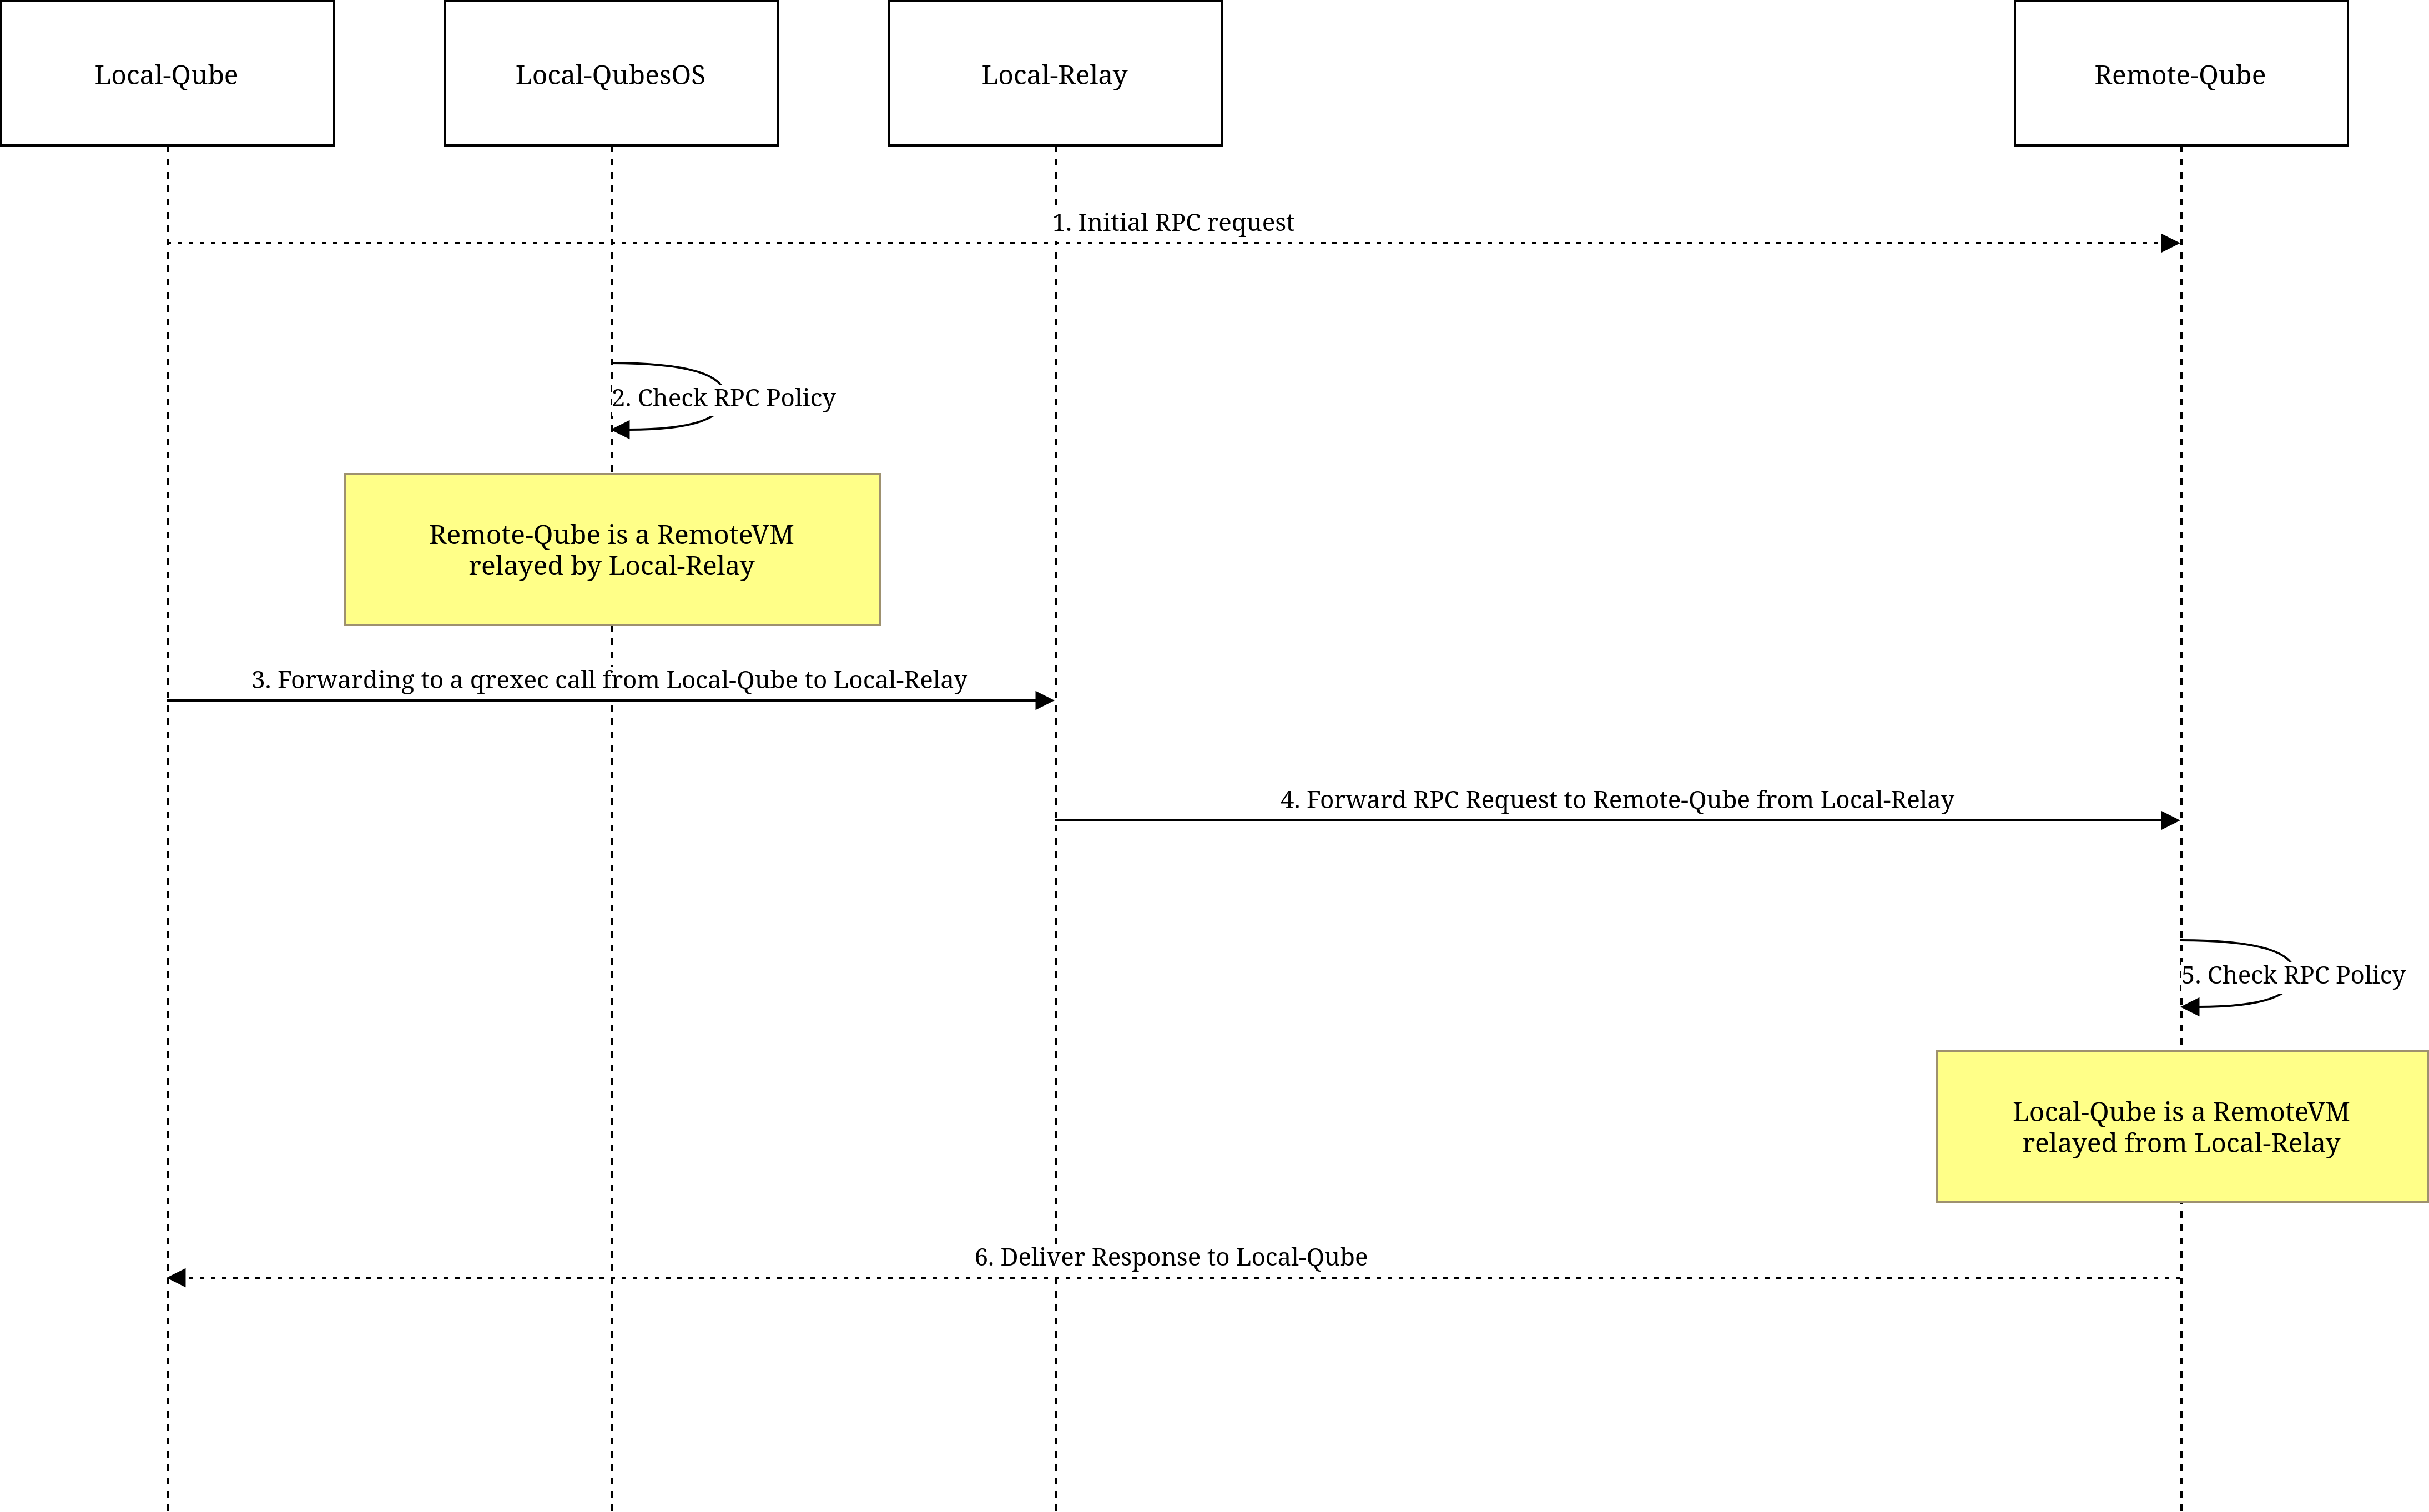
\includegraphics[width=\linewidth]{particular.png}
    \end{center}
\end{frame}

\begin{frame}{Particular Case: Non-QubesOS Host RemoteVM}
    \begin{itemize}
        \item RemoteVM can be on standard Linux or Windows machines, RPi, etc.
        \item Useful for interaction with other virtual machines (e.g. KVM VMs).
		\item Delegate high resource usage to dedicated hosts.
    \end{itemize}
\end{frame}

\begin{frame}{Summary}
    \begin{itemize}
        \item The process involves multiple relays and policy checks to ensure secure communication.
        \item Potential improvements include end-to-end verification and handling of unknown connections.
    \end{itemize}
\end{frame}

\end{document}
